% This is samplepaper.tex, a sample chapter demonstrating the
% LLNCS macro package for Springer Computer Science proceedings;
% Version 2.20 of 2017/10/04
%
\documentclass[runningheads]{llncs}
%
\usepackage{graphicx}
\usepackage{amsmath}
\usepackage{amsfonts}
\usepackage{float}
% Used for displaying a sample figure. If possible, figure files should
% be included in EPS format.
%
% If you use the hyperref package, please uncomment the following line
% to display URLs in blue roman font according to Springer's eBook style:
% \renewcommand\UrlFont{\color{blue}\rmfamily}

\begin{document}
%
\title{Dual watermarking for handwritten document image integrity, tamper detection and copyright protection for JPEG compression attacks}
%
%\titlerunning{Abbreviated paper title}
% If the paper title is too long for the running head, you can set
% an abbreviated paper title here
%
\author{Ernesto Avila-Domenech\inst{1}\orcidID{0000-0002-4797-289X} \and
Alberto Taboada-Crispi\inst{2}\orcidID{0000-0002-7797-1441} \and
Anier Soria-Lorente\inst{1}\orcidID{0000-0003-3488-3094}}
%
\authorrunning{E. Avila-Domenech et al.}
% First names are abbreviated in the running head.
% If there are more than two authors, 'et al.' is used.
%
\institute{Universidad de Granma, Carretera Central v{\'i}a Holgu{\'i}n Km $\frac{1}{2}$, Granma, Cuba \email{\{eadomenech, asorial1983\}@gmail.com}\\ \and
Universidad Central de Las Villas, Villa Clara, Cuba\\
\email{\{ataboada\}@uclv.edu.cu}}
%
\maketitle              % typeset the header of the contribution
%
\begin{abstract}
For the integrity, tamper detection and copyright protection of handwritten document images, a dual watermarking algorithm that connects the robust watermarking algorithm based on Krawtchouk moments with a fragile watermarking algorithm based on MD5 hash function is presented. Hence, the robust watermarking algorithm is used to guarantee robustness by modifying frequency coefficients in Krawtchouk moments. Thus, this study proposes a fragile watermarking algorithm, which can perceive in time when the protected image is tampered. Experimental results show that the proposed algorithm can be used for copyright protection for JPEG compression attacks and tampering detection of this images.

\keywords{Handwritten  \and Image \and Watermarking.}
\end{abstract}
%
%
%
\section{Introduction}
The explosive growth of digital multimedia techniques, together with the rapid development of digital network communication has created a pressing demand for techniques that can be used for copy protection, copyright protection and content authentication. Owing to the need of copyright protection and authentication validation, Digital Rights Management (DRM) is gaining importance. DRM refers to a range of access control technologies used to limit or restrict usage of digital content. Digital watermarking is useful in DRM systems as it can hide information within the digital content like images, audio and video.

Watermarking technique is effectively applied to content authentication, integrity protection, and image copyright. In accordance with the desired robustness of the embedded watermark, digital watermarking techniques are divided into fragile watermarking and robust watermarking. The first ones is designed to detect slight changes to the watermarked image with high probability and the second ones is typically used for copyright protection, thus it is designed to resist attacks that attempt to remove or destroy the watermark without significantly degrading the visual quality of the watermarked image.

When users want to detect illegal tampering and at the same time protect the copyright, the single watermarking algorithm cannot meet the needs of users. Therefore, the double watermarking algorithm is developed, as it can effectively combine the advantages and functions of the two watermarks \cite{wang2017dual}.

Numerous double watermarking algorithms have been proposed. In \cite{mohanty1999dual} is presented a dual watermarking technique which attempts to establish the owner’s right to the image and detect the intentional and unintentional tampering of the image. However, this early research is simply a combination of visible and invisible watermarking algorithms. In \cite{wang2017dual} is presents a dual watermarking algorithm that connects the robust watermarking algorithm based on singular value decomposition (SVD) with a fragile watermarking algorithm based on compressive sensing (CS). In \cite{singh2018hybrid} use cryptography and QR Code in combined approach of LSB and DCT Digital image watermarking technique, it combines the LSB and DCT approach because LSB contain spatial domain property and DCT contain frequency domain property.

In \cite{shivani2017dual} provides dual functionalities of ownership assertion and authentication. In \cite{liu2018blind} presents a blind dual watermarking mechanism for digital color images. The first watermark is embedded by using the discrete wavelet transform (DWT) in YCbCr color space, and it can be extracted blindly without access to the host image. However, fragile watermarking is based on an improved least significant bits (LSB) replacement approach in RGB components for image authentication. In \cite{singh2019robust} presents lifting wavelet transform (LWT) and discrete cosine transform (DCT) based robust watermarking approach for tele-health applications. They are based on LWT requires less memory, reduced aliasing effects and distortion, fast and it is a good choice for low computational complexity than conventional DWT.

The rest of the paper is organized as follow; Section 2 describes the proposed method including robust watermarking and fragile watermarking. Experimental results are given in Section 3 and Section 4 concludes the paper.

\section{Proposed method}
Dual watermarking implies embedding of robust as well as fragile watermarks into the same cover image. It facilitates integration of copyright protection and integrity verification into the same scheme. First robust watermarking and then the fragile watermarking should be done because the fragile watermarking is sensitive to small changes. Unlike the fragile watermarking, robust resists changes caused by performing the marked fragile.
\begin{figure}
	\begin{center}
		\includegraphics[width=\textwidth]{dual_watermarking.png}
		\caption{Dual watermarking scheme.} \label{dual_watermarking}
	\end{center}
\end{figure}

\subsection{Robust watermarking}
The robust watermarking method proposed is similar to the one proposed in \cite{avila2018watermarking}. The difference consists in ...

The following steps are taken to embedding process:
\begin{enumerate}
	\item The binary watermark image (QR code) is scrambled using Arnold transform \cite{Arnol'd:1987366}.
	\item The cover image is transformed from RGB to YCbCr color space, and the Y component, corresponding to the luminance information, is divided into small image blocks of $8\times 8$ pixels.
	\item A number of blocks equal to the number of bits to be inserted is selected from a given key.
	\item Each selected block is classified by the model previously trained in one of the defined classes.
	\item The Krawtchouk moments \cite{Yap2003} of selected blocks are determined.
	\item Watermark bit is embedded in the selected block moments using Dither modulation \cite{chen2001quantization}. Both the coefficient and embedding strength values are obtained according to the class that has been classified each block. Watermarked blocks can be obtained. 
	\item Transform the YCbCr to RGB color space to obtain RGB watermarked image.
\end{enumerate}

For watermark extraction:
\begin{enumerate}
	\item The watermarked image is transformed from the RGB to the YCbCr color space and the Y component is divided into $8\times 8$ pixels blocks.
	\item Some blocks are selected from which they will be extracted from the key used in the embedding process.
	\item Each selected block is classified by the model previously trained in one of the defined classes. According to the class, the coefficient and embedding strength values to be used in the extraction are determined.
	\item The Krawtchouk moments of selected blocks are determined.
	\item Scrambled watermark bits are obtained with the selected blocks moments using Dither modulations.
	\item Finally, QR code watermark is constructed with the scrambled bits using Arnold transform.
\end{enumerate}

\subsection{Fragile watermarking}
As we know, hash function, such as MD5 or SHA-256, can be utilized to authenticate the data integrity. If the hash value of original message is exactly equal to the re-calculated hash value of the received message, the received data can be regarded as integrated, otherwise as false.

For the process of embedding the following steps are performed:
\begin{enumerate}
	\item The RGB image is divided into $32\times 32$ non-overlapped blocks.
	\item 128 pixels of each block are selected by a given key.
	\item The least significant bits (LSBs) of each selected pixel are assigned the value 0.
	\item The MD5 hash value of the modified block is generated as a watermark.
	\item The watermark is embedded into the LSBs of the selected pixels and watermarked block image is obtained.  
\end{enumerate}    

The detection of a fragile watermark is the inverse process of watermark generation, which is used to detect whether the watermarked image has been tampered and what the precise position of the tampered parts is. For this:
\begin{enumerate}
	\item The RGB image is divided into $32\times 32$ non-overlapped blocks.
	\item 128 pixels of each block are selected by a given key.
	\item Three binary series are formed from the LSBs of the selected pixels.
	\item The LSBs of each selected pixel are assigned the value 0.
	\item The MD5 hash value of the modified block is generated and compareted with obtained series.
\end{enumerate}

\section{Experiments and Results}
The watermarking algorithm is evaluated through imperceptibility, tamper detection and robustness, and the following experiments are introduced.

We used two handwriten document image databases: Saint Gall \cite{fischer2011transcription} and Parzival \cite{fischer2009automatic} database. The first one contains manuscripts from the 9th century using Carolingian scripts by a single writer, while the Parzival is compiled from 13th century Gothic scripts \cite{pastor2016complete}.
 

\subsection{Imperceptibility}
The imperceptibility of the watermark was evaluated using several databases. We calculated the larger peak signal to noise ratio (PSNR) which compares the similarity between the original image $ I $ and the watermarked image $ I_w $. A PSNR indicates that the watermarked image more closely resembles the original image meaning that the watermark is more imperceptible. (see Fig.~\ref{psnr})
\begin{figure}[H]
	\begin{center}
		\begin{tabular}{|c|c|}\hline
			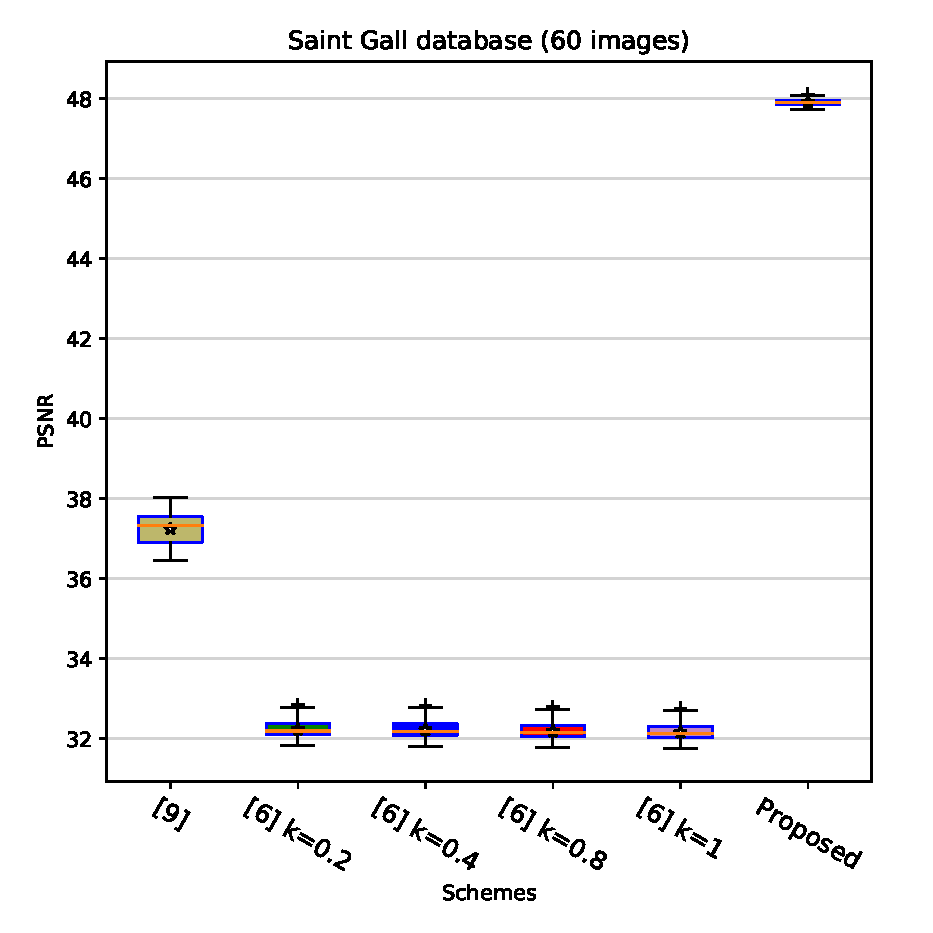
\includegraphics[width=0.5\textwidth]{PSNR_saintgall.eps}
			&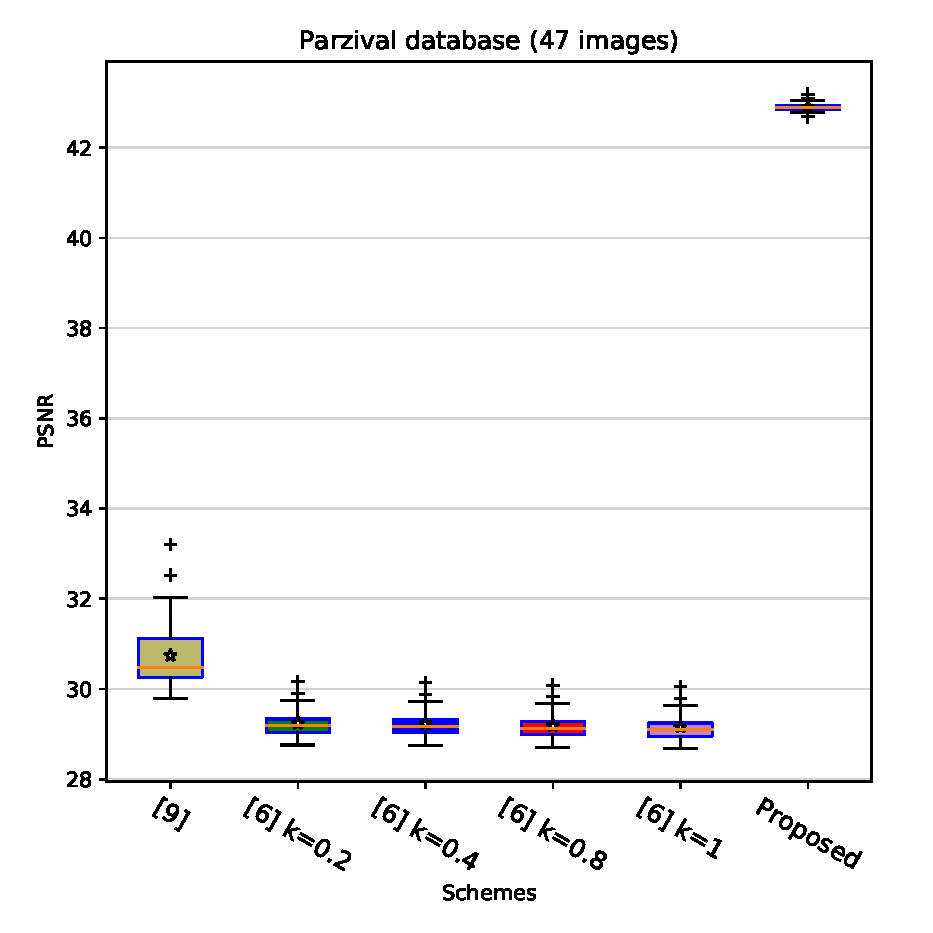
\includegraphics[width=0.5\textwidth]{PSNR_parzival.eps}\\\hline
		\end{tabular}
	\end{center}
	\caption{PSNR values for Saint Gall database watermarked images.}
	\label{psnr}
\end{figure}

\subsection{Tamper detection}
Tamper area detection capability is evaluated, by modifying the contents of images, adding objects or deleting objects. We developed our proposed fragile watermarking particularly for integrity images and locating tampered areas. Fig. 7 shows the attacked images and their corresponding tamper detection results, where N MP represents the total number of modified pixels in the tampered image, N P is the number of detected pixels, and accurate rate (AR) is the percentage of detected pixels in modified pixels.
\begin{figure}[H]
	\begin{center}
		\begin{tabular}{|c|c|c|c|}\hline
			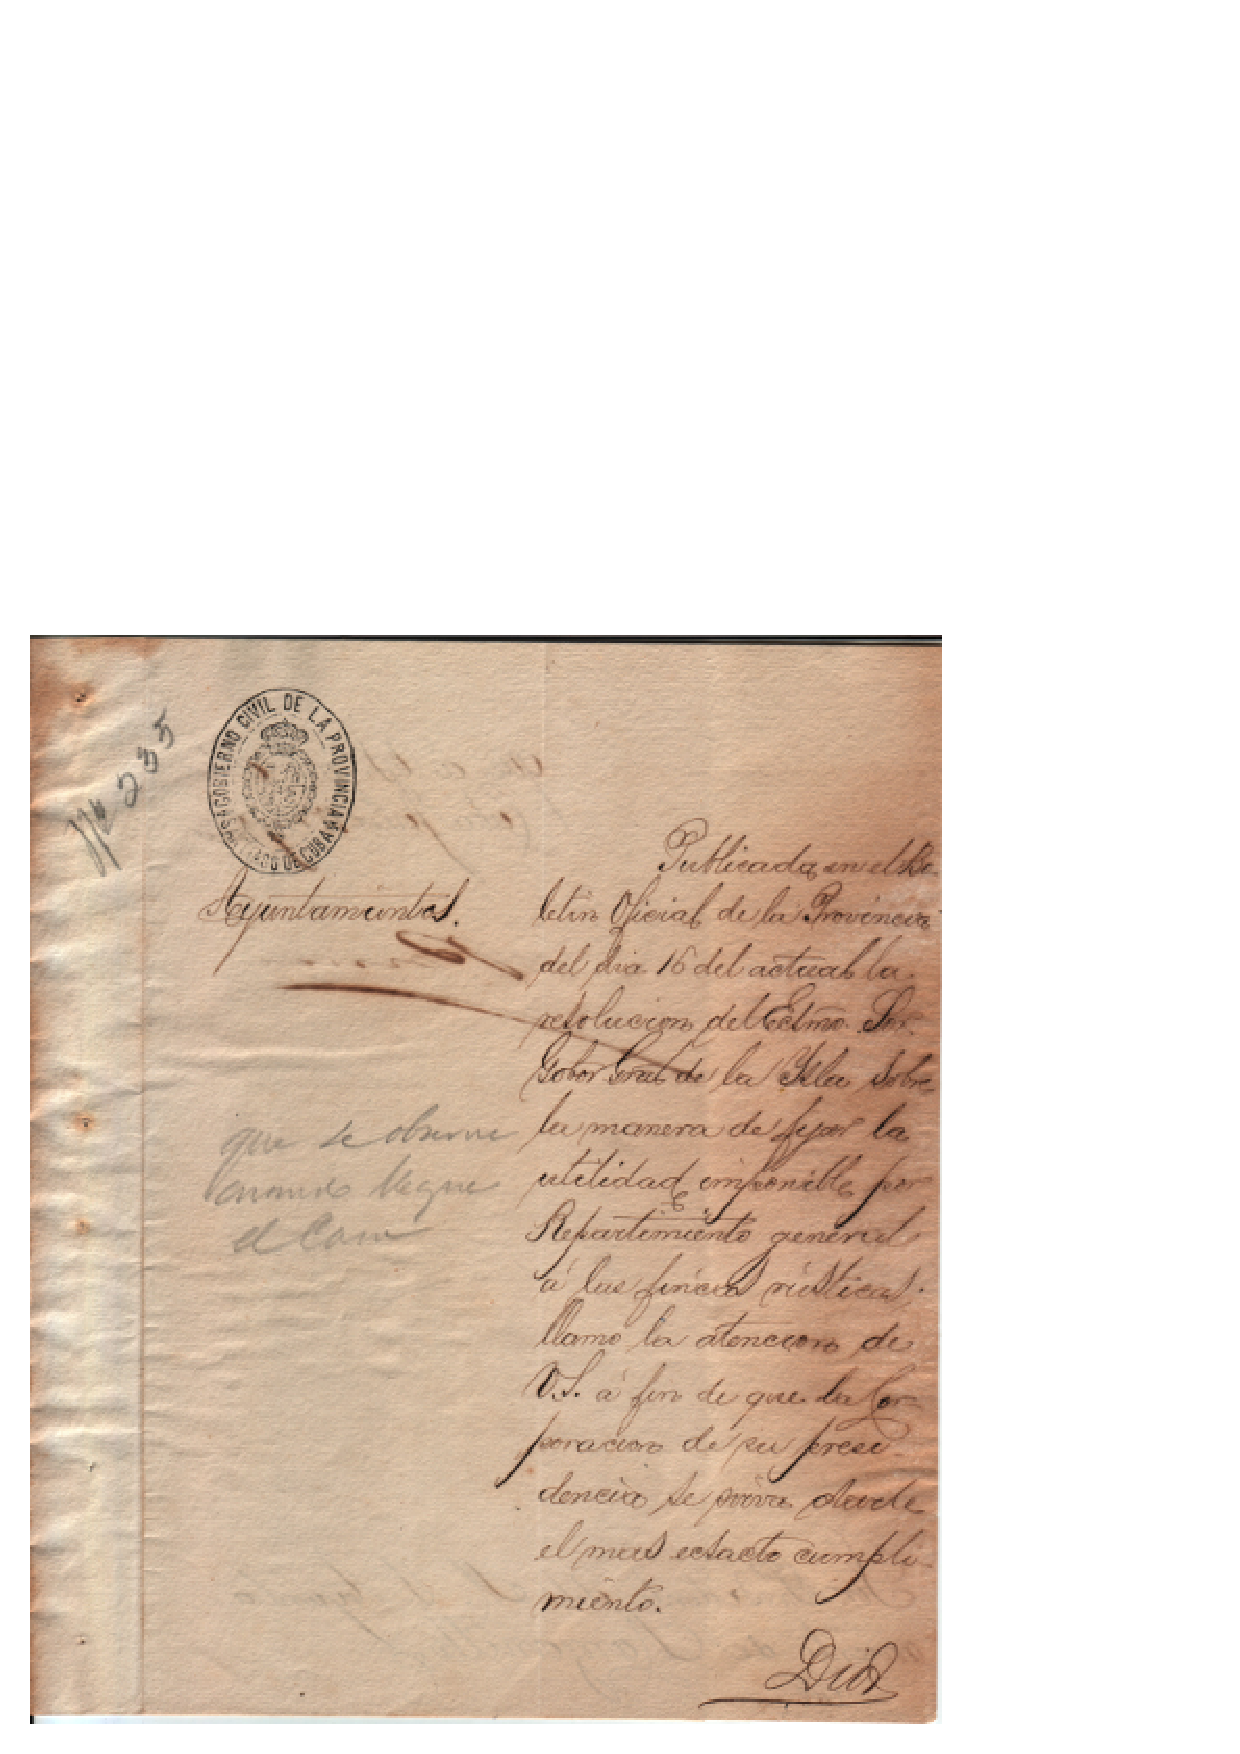
\includegraphics[width=0.25\textwidth]{1.jpg}
			&\includegraphics[width=0.25\textwidth]{watermarked_image.png}
			&\includegraphics[width=0.25\textwidth]{watermarked_image_with_noise.png}
			&\includegraphics[width=0.25\textwidth]{tampered_image.png}\\\hline
		\end{tabular}
	\end{center}
	\caption{Original image, watermarked image, modified watermarked image and tamper area detection.}
	\label{img_of_AHM}
\end{figure}
\subsection{Robustness}
The bit error rate (BER) is defined as ratio between number of incorrectly decoded bits and total number of bits.
\begin{figure}[H]
	\begin{center}
		\begin{tabular}{|c|c|}\hline
			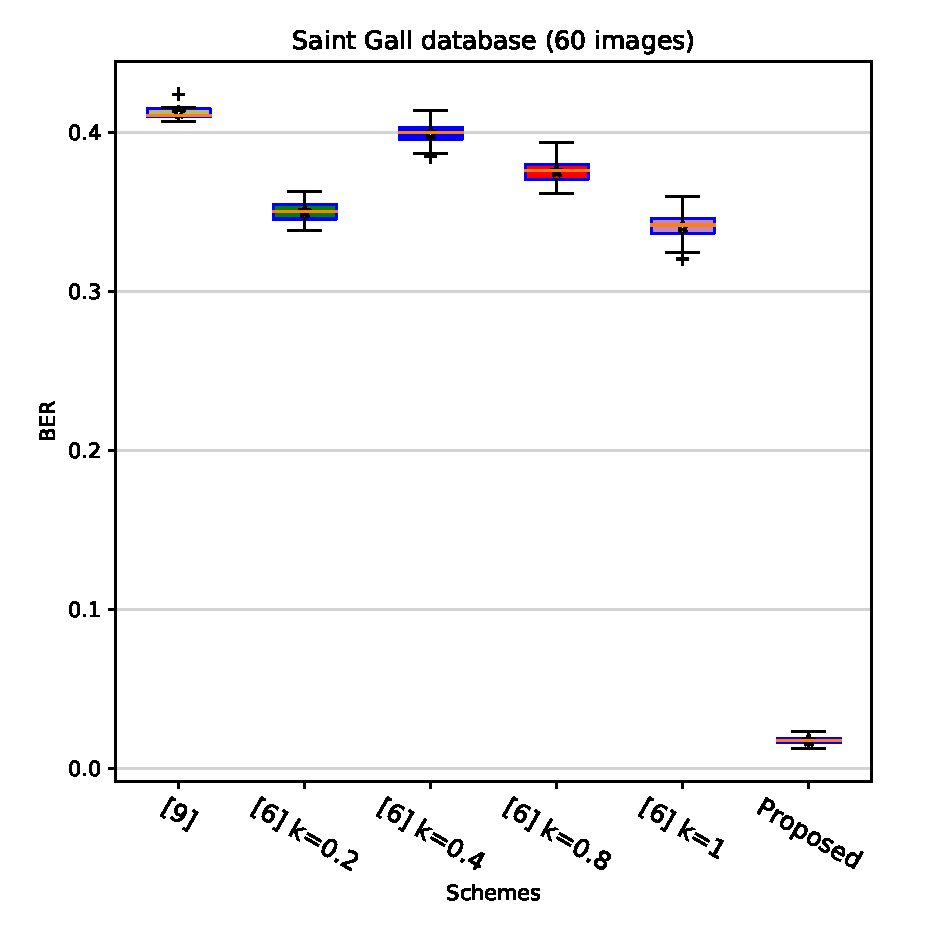
\includegraphics[width=0.5\textwidth]{BERWithoutSaintGall.eps}
			&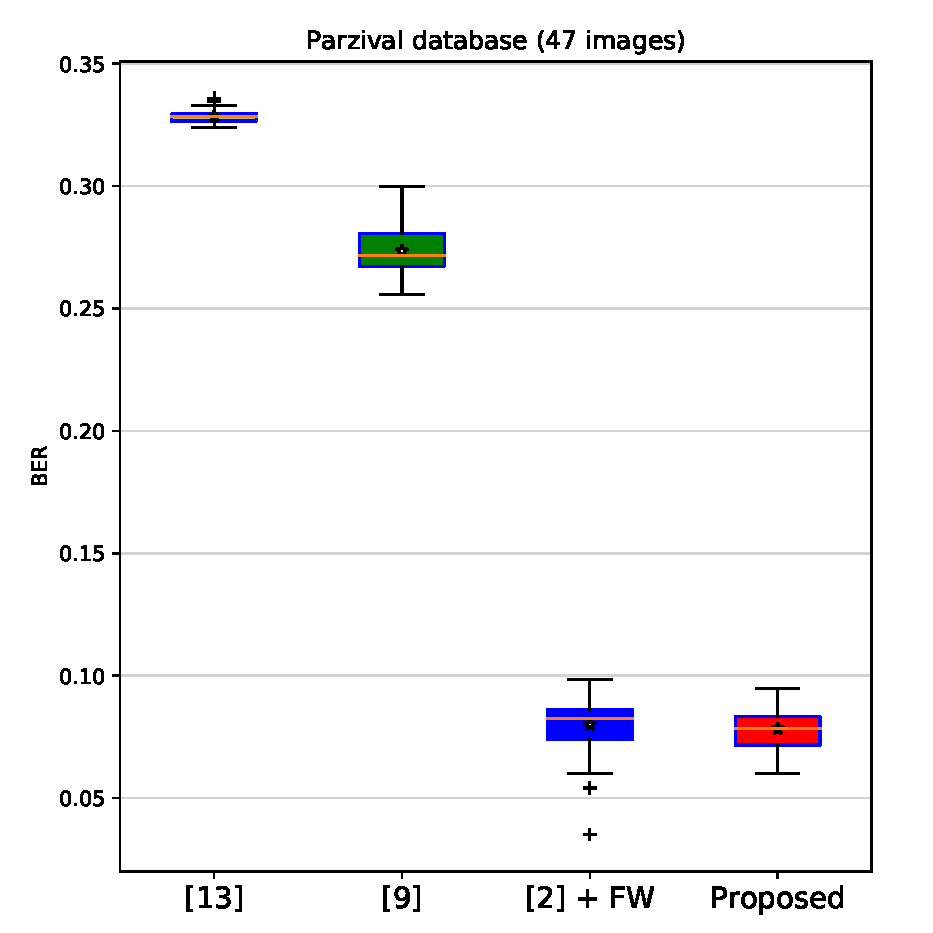
\includegraphics[width=0.5\textwidth]{BERWithoutParzival.eps}\\\hline
		\end{tabular}
	\end{center}
	\caption{BER values for watermarked images without noise.}
	\label{berWithout}
\end{figure}
\begin{figure}[H]
	\begin{center}
		\begin{tabular}{|c|c|}\hline
			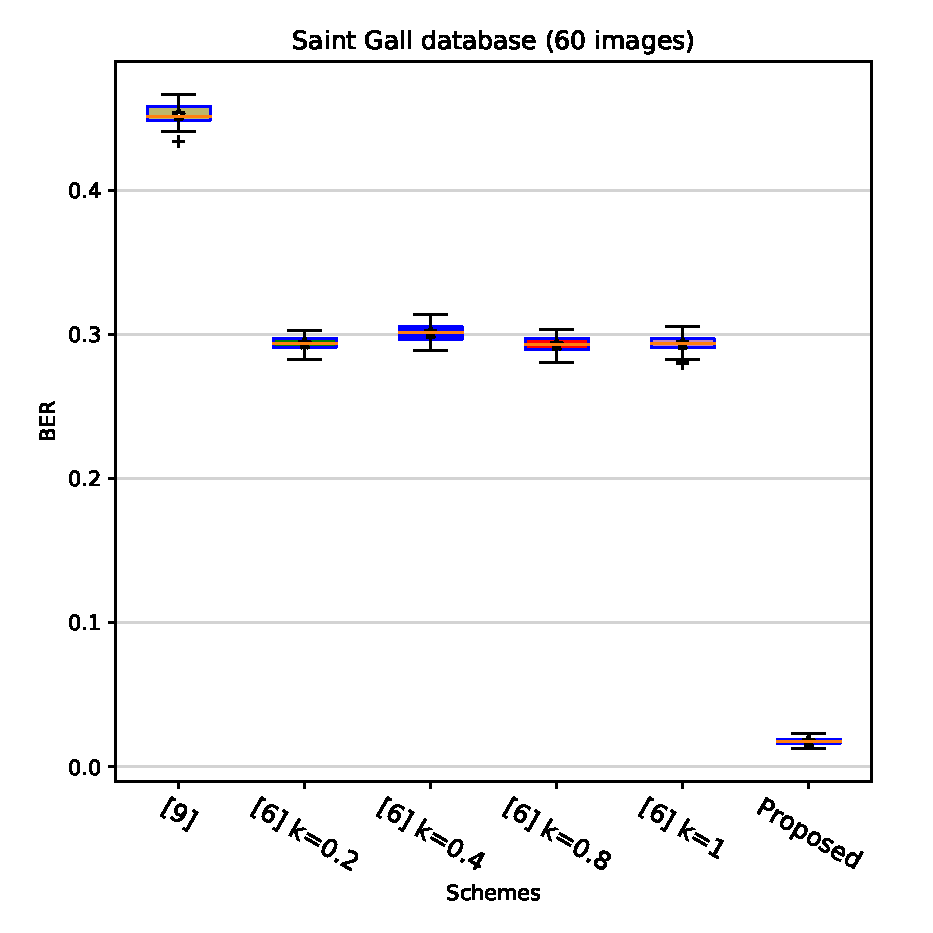
\includegraphics[width=0.5\textwidth]{BER75SaintGall.eps}
			&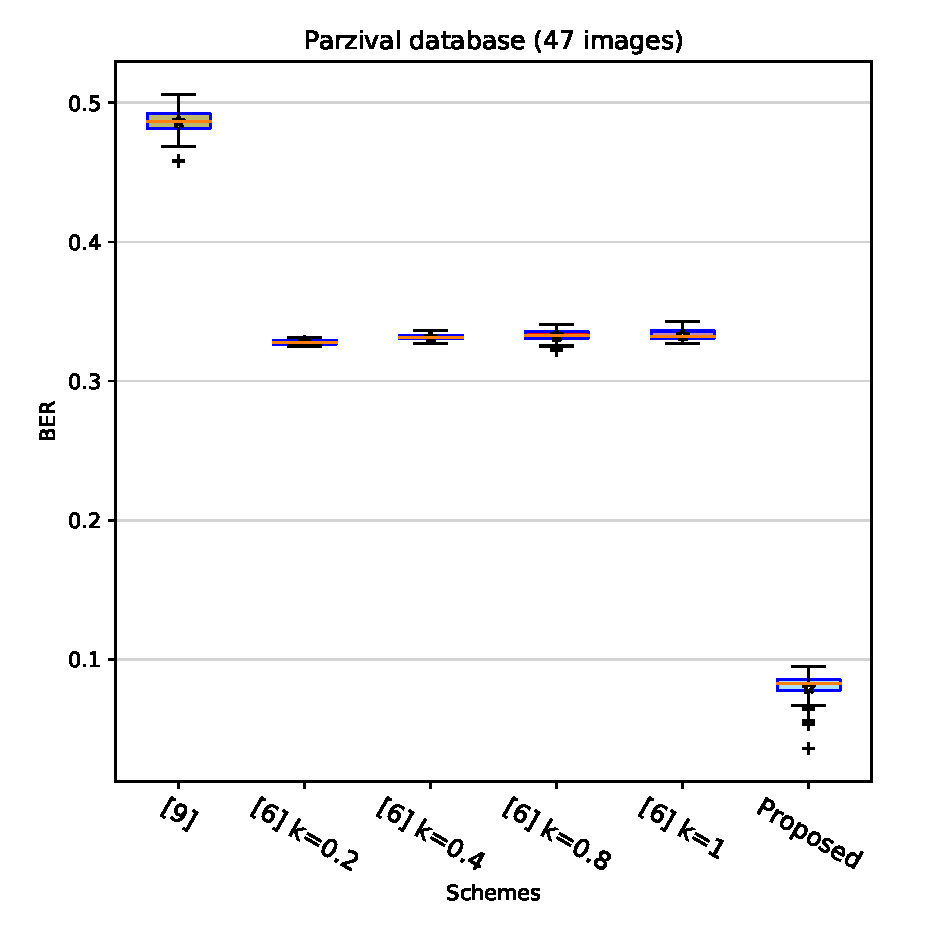
\includegraphics[width=0.5\textwidth]{BER75Parzival.eps}\\\hline
		\end{tabular}
	\end{center}
	\caption{BER values for watermarked images with JPEG compression (QF=75\%).}
	\label{ber75}
\end{figure}
\begin{figure}[H]
	\begin{center}
		\begin{tabular}{|c|c|}\hline
			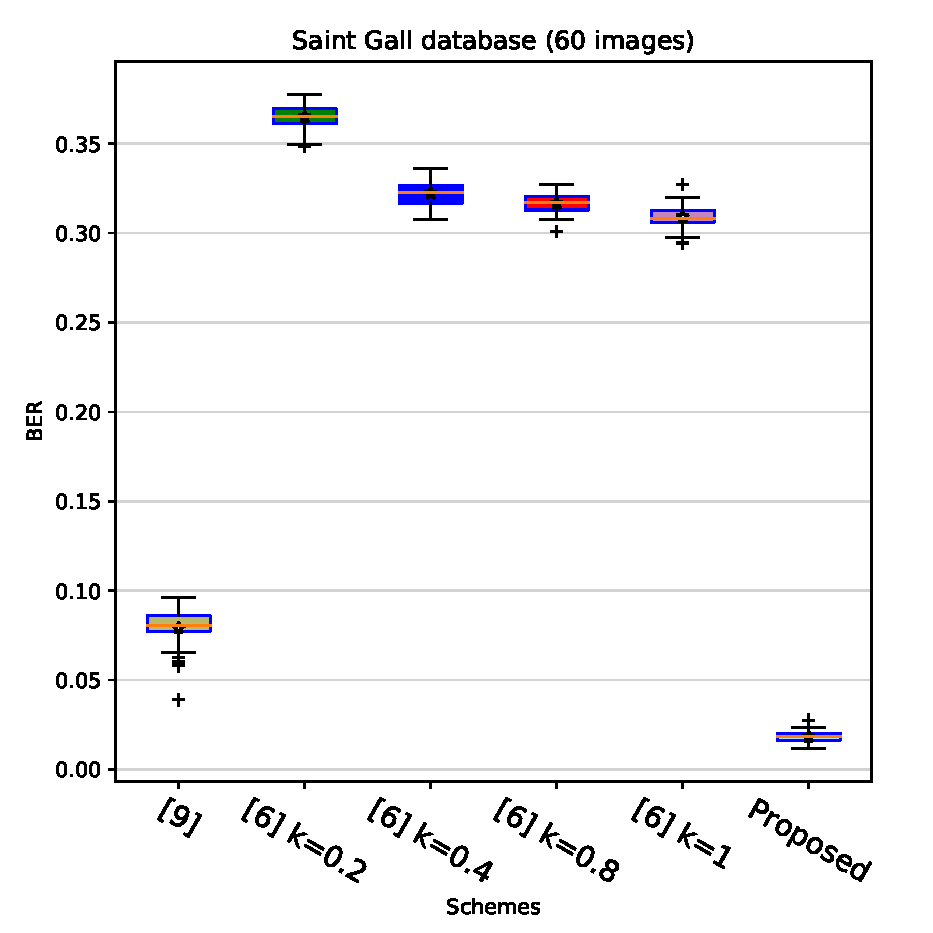
\includegraphics[width=0.5\textwidth]{BER50SaintGall.eps}
			&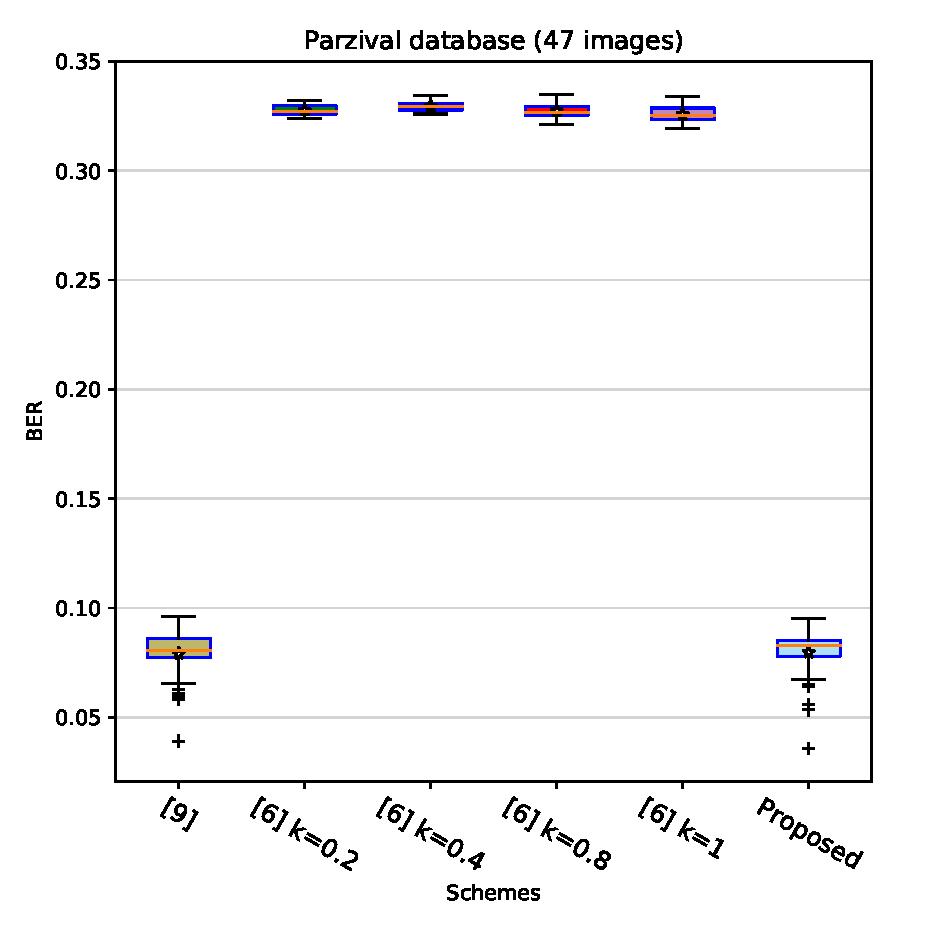
\includegraphics[width=0.5\textwidth]{BER50Parzival.eps}\\\hline
		\end{tabular}
	\end{center}
	\caption{BER values for watermarked images with JPEG compression (QF=50\%).}
	\label{ber50}
\end{figure}
\begin{figure}[H]
	\begin{center}
		\begin{tabular}{|c|c|}\hline
			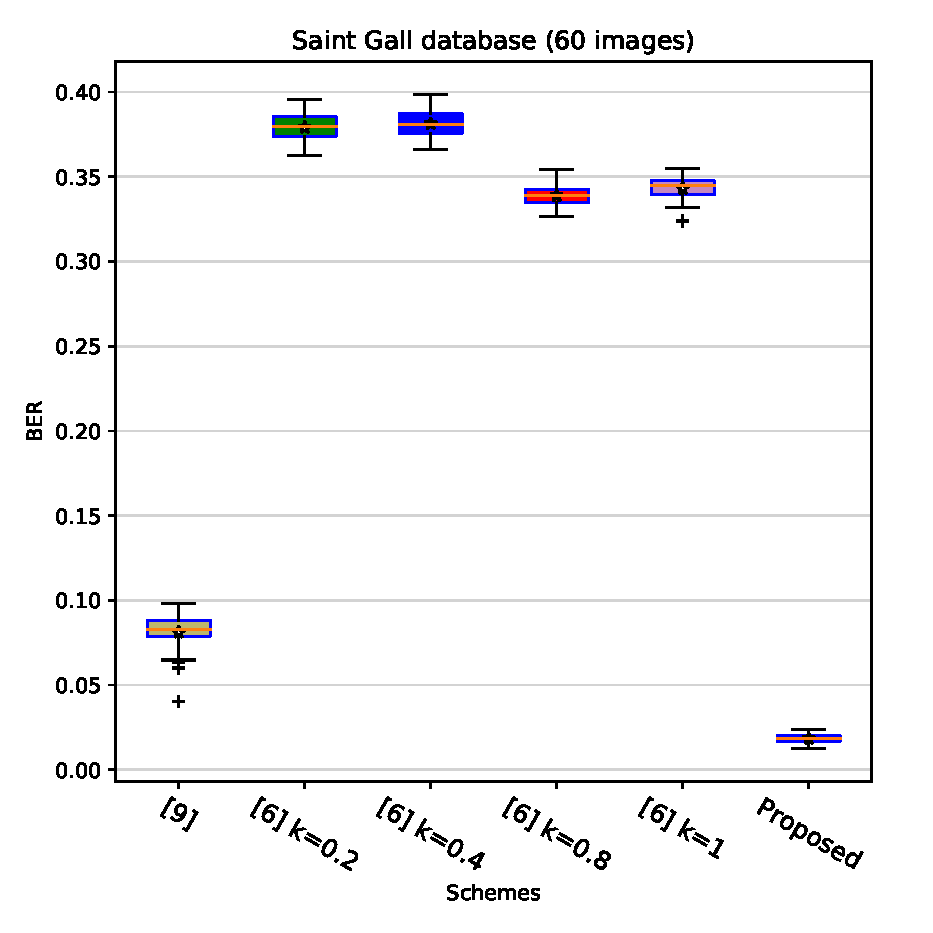
\includegraphics[width=0.5\textwidth]{BER25SaintGall.eps}
			&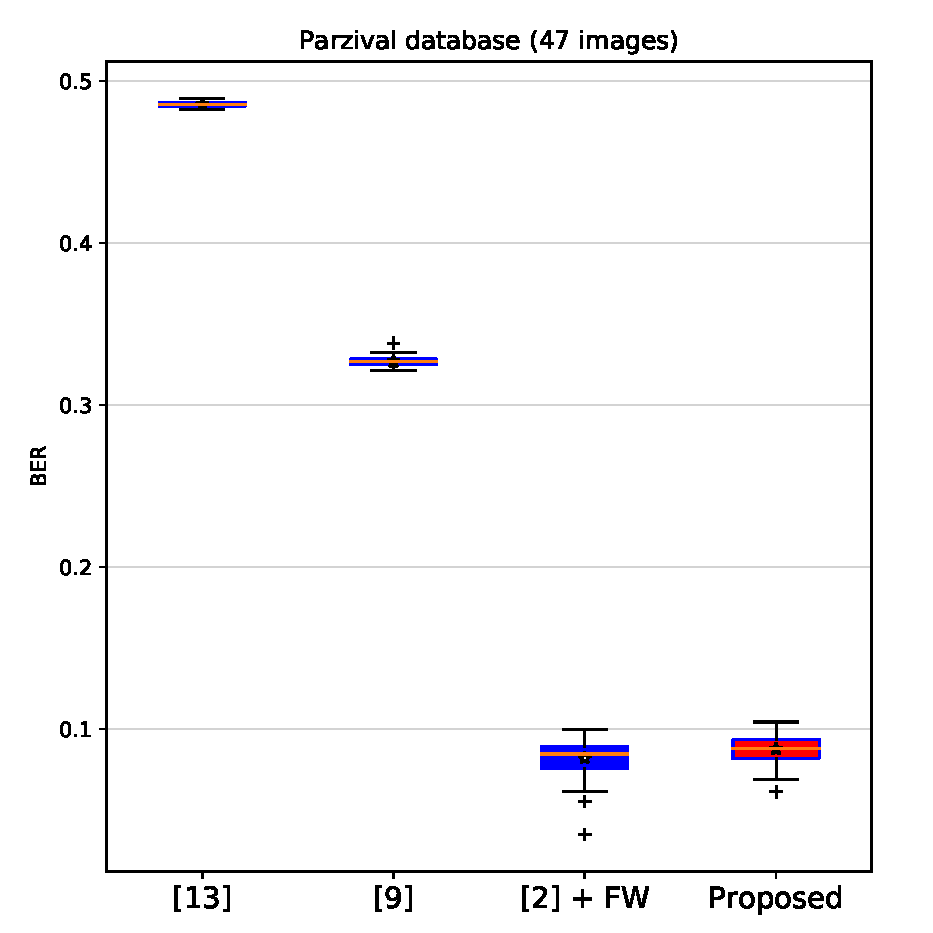
\includegraphics[width=0.5\textwidth]{BER25Parzival.eps}\\\hline
		\end{tabular}
	\end{center}
	\caption{BER values for watermarked images with JPEG compression (QF=25\%).}
	\label{ber25}
\end{figure}

\section{Conclusions}
In this paper, a dual digital watermarking technique based on Krawtchouk moments and MD5 hash function was implemented. The results show a BER less than $0.006 \%$, so the extracted QR codes were decoded in $100\%$ of the $60$ analyzed images. In addition, the values corresponding to the PSNR were improved compared to previously presented papers.
%
% ---- Bibliography ----
%
% BibTeX users should specify bibliography style 'splncs04'.
% References will then be sorted and formatted in the correct style.
%
\bibliographystyle{splncs04}
\bibliography{mybibliography}
%
\end{document}
